\clearpage
\setcounter{page}{1}
\maketitlesupplementary

\begin{figure*}[h]
    \centering
    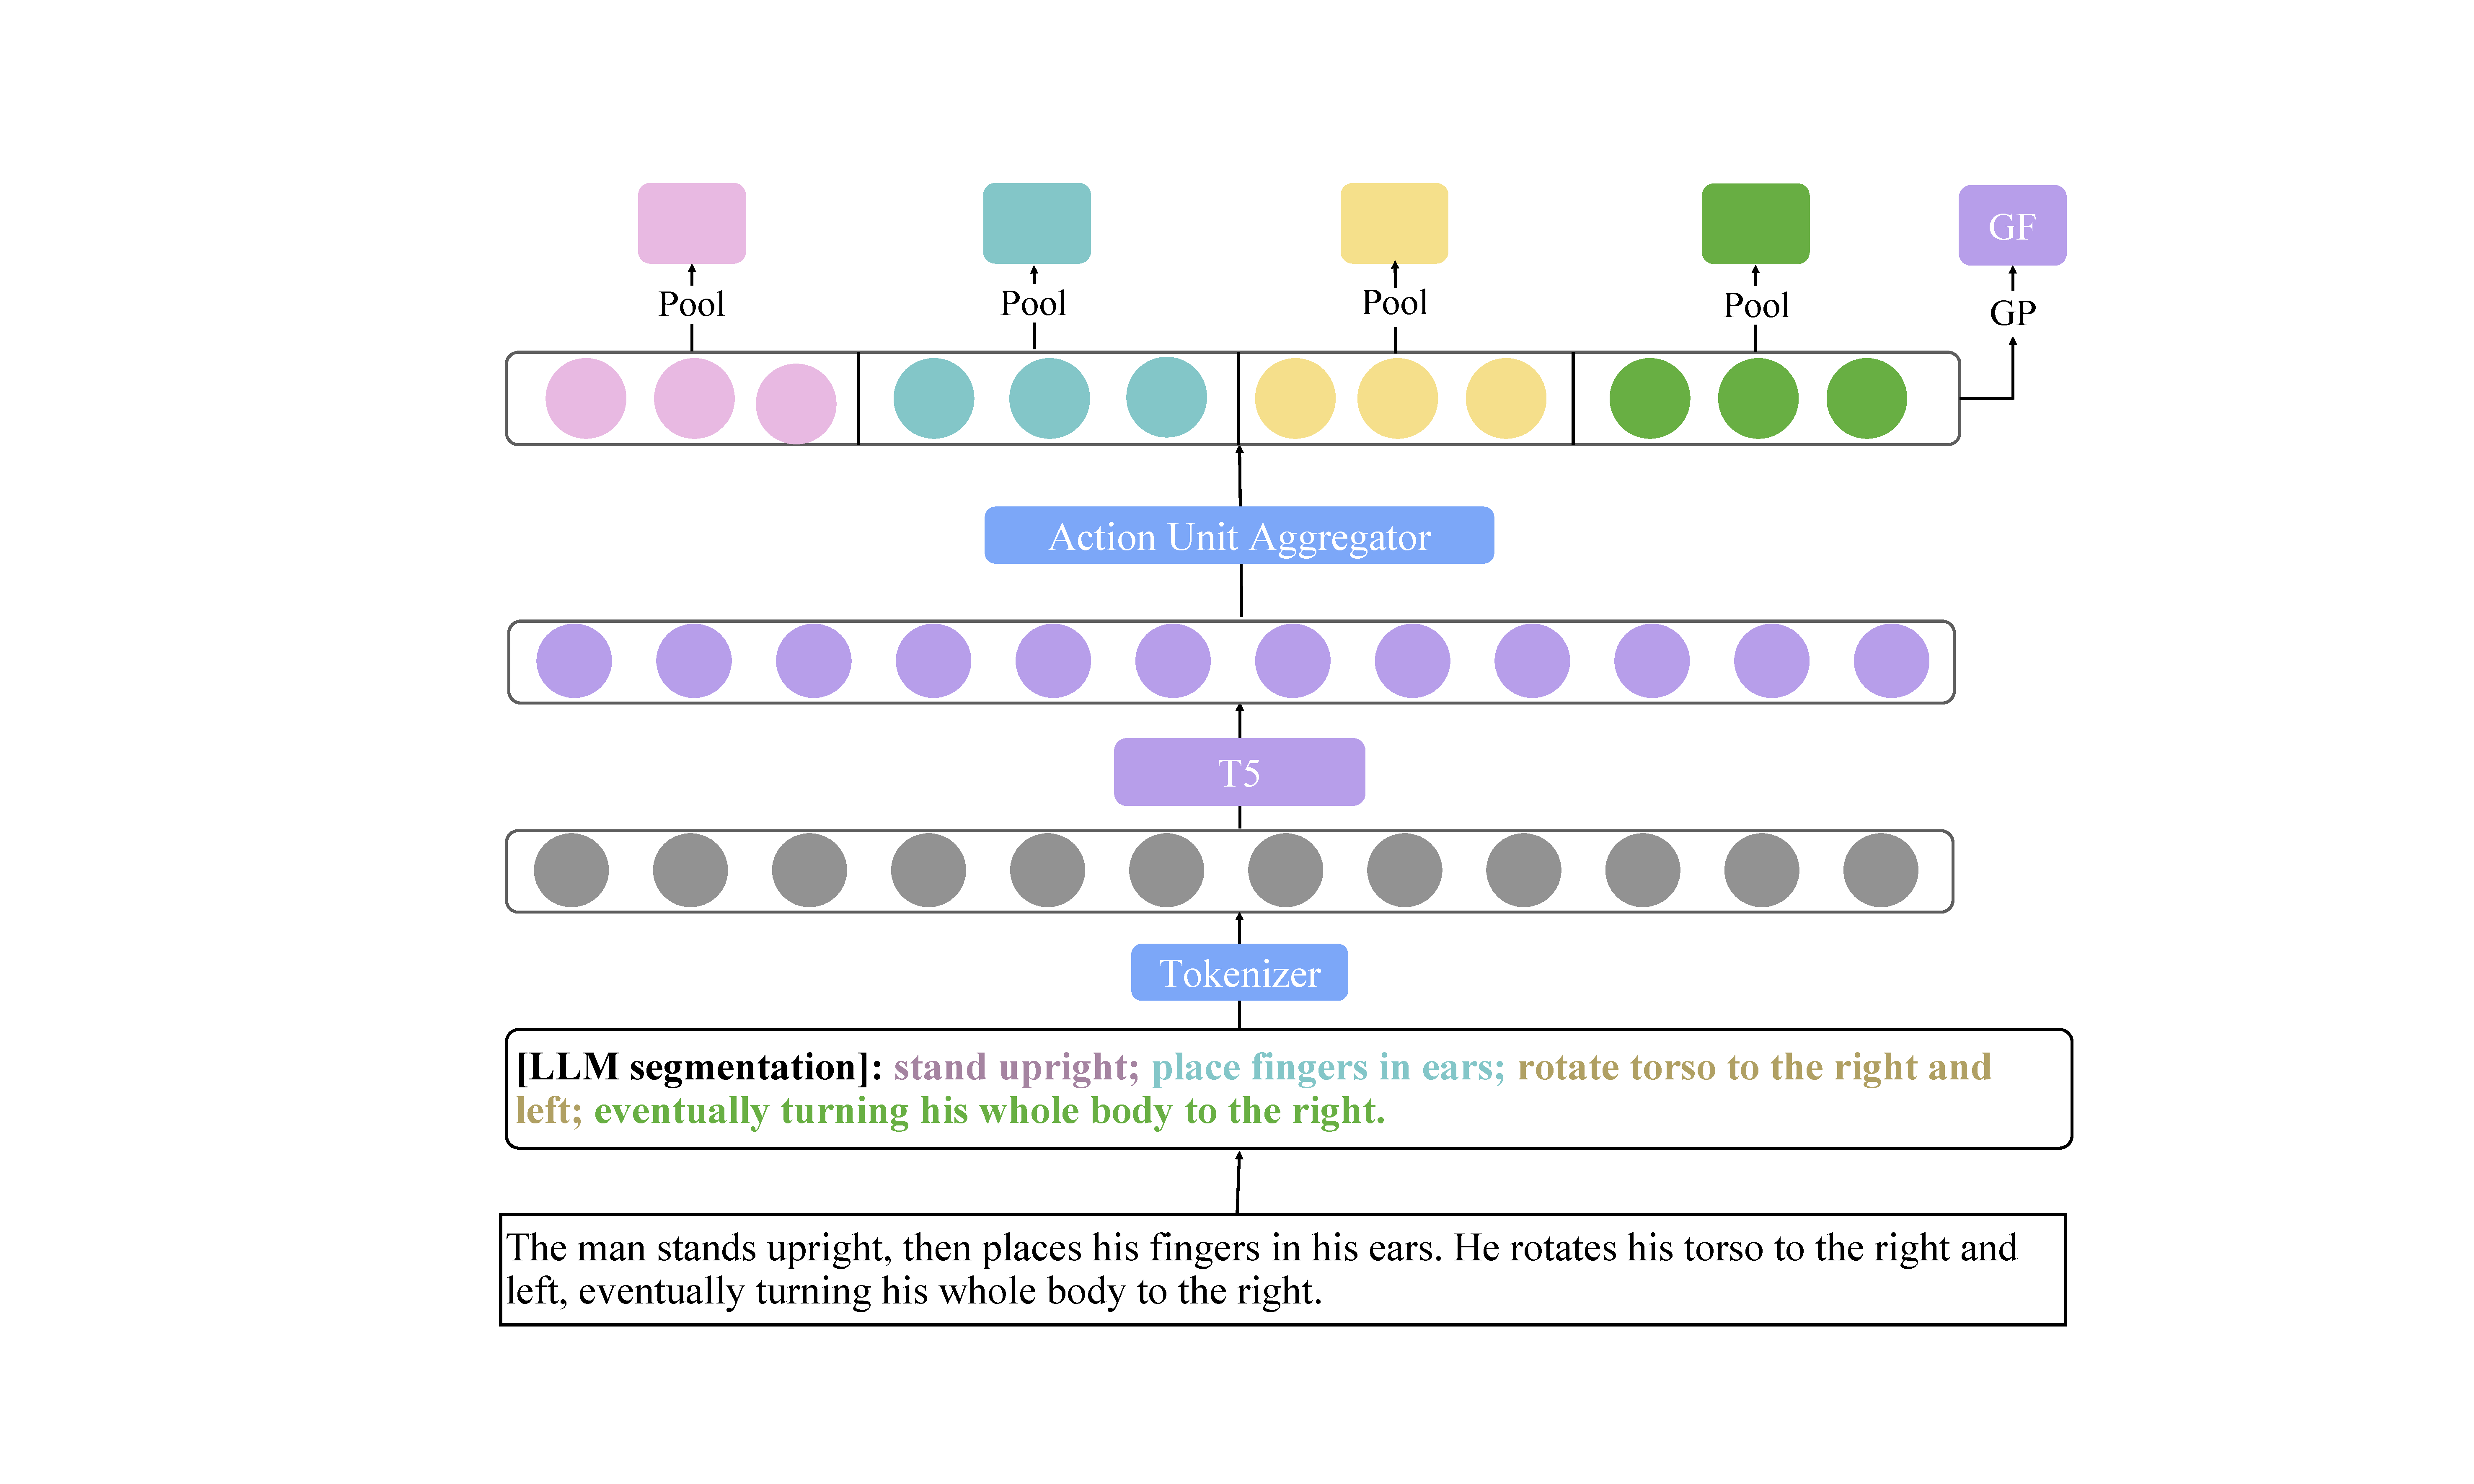
\includegraphics[width=\linewidth]{author-kit-CVPR2026-v1-latex-/figs/ActionAggregator.pdf}
    \caption{
Overview of the \textbf{action unit aggregator}. 
A long-form motion caption is first segmented into multiple \textbf{action-bearing phrases} using an LLM. 
The concatenated phrase sequence is tokenized and encoded by a frozen T5 backbone to obtain token-level embeddings. 
The action unit aggregator then groups tokens belonging to the same phrase and pools them into compact \textbf{action unit features}. 
An additional \textbf{global feature} (GF) is obtained by global pooling (GP) over the entire sequence, which acts as an \texttt{[UNK]} token to absorb motion frames that are not explicitly described by any phrase.}
    \label{fig:aggre}
\end{figure*}

\section{Proof of Theorem 1}
\begin{theorem}[Zero OT Cost under Perfect Alignment]
\label{thm:zero_ot}
Under Assumption 1, the OT objective $\mathcal{J}_{OT}(m,t)$ admits a feasible transport plan with zero cost. Specifically, the transport plan defined by
\begin{equation}
P_{uv}=\frac{1}{T_m}\mathbbm{1}\{v=\pi(u)\}
\end{equation}
is feasible and achieves
\begin{equation}
\mathcal{J}_{OT}(m,t)=0.
\end{equation}
\end{theorem}

\begin{proof}
Under Assumption 1, for each motion frame $u$, there exists a unique text token $\pi(u)$ such that
$s(z^m_u,z^t_{\pi(u)})=1$.
By Eq. 7, this implies that $\mathbf{C}_{u,\pi(u)}=0$.
Now consider the transport plan
\begin{equation}
P_{uv}=\frac{1}{T_m}\mathbbm{1}\{v=\pi(u)\}.
\end{equation}
Since $\pi$ is a bijection and $T_m=T_t$, each row and each column of $P$ contains exactly one nonzero entry equal to $1/T_m$. Therefore, $P$ satisfies the marginal constraints and is feasible. The total transport cost is
\begin{equation}
\sum_{u=1}^{T_m}\sum_{v=1}^{T_t} P_{uv}\mathbf{C}_{uv}=0,
\end{equation}
which is the minimum possible value. Hence, $\mathcal{J}_{OT}(m,t)=0$.
\end{proof}
\section{Caption Segmentation}
To bridge the gap between long-form narrative descriptions and local temporal motion segments, we first decompose each caption into multiple \textbf{action-bearing phrases} using an LLM-based caption segmentation pipeline, as illustrated in \cref{fig:aggre}. 
Specifically, GPT-4o-mini rewrites each caption into a sequence of semicolon-separated phrases, where each phrase describes a temporally coherent action while preserving the original temporal order. The prompt is illustrated in \cref{fig:segmentation_prompt}.

The segmented phrases are concatenated and processed by a tokenizer and a frozen T5 encoder to obtain token-level embeddings. 
We then apply the \textbf{action unit aggregator}, which identifies token spans corresponding to each phrase using separator tokens (``\texttt{;}'') and the end-of-sequence token. 
For each span, token embeddings are pooled along the sequence dimension to produce compact \textbf{action unit features}.

In addition, we compute a \textbf{global features} by pooling over the entire token sequence. 
This global feature acts as an \texttt{[UNK]} token that absorbs motion frames not explicitly described by any phrase. 
The final text feature set, therefore, consists of the action unit features together with the global feature, which are used for the Sinkhorn-based motion–text alignment described in the main paper.

\begin{figure*}[h]
\begin{mdframed}[backgroundcolor=gray!10, roundcorner=5pt, innertopmargin=10pt, innerbottommargin=10pt, innerrightmargin=10pt, innerleftmargin=10pt]
{\small
\textbf{System Prompt}  \vspace{0.5em}
You are an expert in Motion Capture (MoCap) and computer animation. Your task is to segment complex motion captions into "Atomic Action Units" to facilitate temporal alignment for motion generation models (e.g., SnapMoGen).
 \vspace{0.5em}
 
\textbf{Segmentation Principles:}
\begin{enumerate}
    \item \textbf{Atomization with Temporal Context:} Break down complex sentences into basic, physically continuous atomic actions.
    \item \textbf{Preserve Sequence Markers:} Keep important temporal markers like "then", "soon after", "finally", or "subsequently" at the beginning of descriptions to provide directionality for alignment.
    \item \textbf{Handle Concurrency:} If actions happen simultaneously (e.g., "while", "during"), include concurrency keywords in the description (e.g., "wave right hand while walking") to signify temporal overlap.
    \item \textbf{Body-part Decoupling:} Separate concurrent movements of different body parts if they are distinct actions.
    \item \textbf{Standardization:} Output must be a structured JSON array of objects.
\end{enumerate}  \vspace{0.5em}
\textbf{Output Format Requirement:} Always return a pure JSON object containing a key \texttt{"results"} which is a list of objects, each with \texttt{"caption\_index"} and \texttt{"atomic\_actions"} (list of objects with \texttt{"id"} and \texttt{"description"}).
 
 \vspace{0.5em}
\hrule
 \vspace{0.5em}

\textbf{Few-Shot Examples} \vspace{0.5em}

\textbf{Example Input Captions to Split:}
\begin{itemize}
    \item "The person walks forward a few steps, pauses, and then steps to her left with her left foot, standing still. She raises her arms slightly in front of her at stomach height before lowering them. She repeats the side step with her left foot and turns her head to the left."
    \item "The person stands with hands raised while slowly nodding their head, then starts to move his hands down while tilting his body forward."
    \item "The person advances quickly, bending at the waist during the walk to pick up an object, then finally stands upright while gazing at the object."
\end{itemize}
% \vspace{0.5em}

\textbf{Example Segmentation Results:}
\begin{verbatim}
{
  "results": [
    {
      "caption_index": 1,
      "atomic_actions": [
        {"id": 1, "description": "walk forward a few steps"},
        {"id": 2, "description": "pause and stand still"},
        {"id": 3, "description": "then step to the left with left foot"},
        {"id": 4, "description": "standing still again"},
        {"id": 5, "description": "raise arms slightly to stomach height"},
        {"id": 6, "description": "soon after, lower arms"},
        {"id": 7, "description": "repeat side step with left foot"},
        {"id": 8, "description": "simultaneously turn head to the left"}
      ]
    },
    {
      "caption_index": 2,
      "atomic_actions": [
        {"id": 1, "description": "stand with hands raised"},
        {"id": 2, "description": "slowly nod head while standing"},
        {"id": 3, "description": "then start to move hands down"},
        {"id": 4, "description": "tilt body forward while moving hands"}
      ]
    },
    {
      "caption_index": 3,
      "atomic_actions": [
        {"id": 1, "description": "advance quickly"},
        {"id": 2, "description": "bend at the waist while walking to pick up object"},
        {"id": 3, "description": "then finally stand upright"},
        {"id": 4, "description": "gaze at the object while standing"}
      ]
    }
  ]
}
\end{verbatim}
}
\end{mdframed}
\caption{The complete system prompt and contextual few-shot examples provided to the LLM for atomic action units segmentation.}
\label{fig:segmentation_prompt}
\end{figure*}
\section{Ground Truth Annotation} 
To quantitatively evaluate the temporal alignment performance, we manually label the ground truth alignment matrix $\mathbf{P}^{gt} \in \mathbb{R}^{T_m \times T_t}$. The annotation process involves manual segment-level boundary identification: for each action segment $j$, human annotators specify the temporal interval $[t_{start}, t_{end}]$ in seconds. These intervals are subsequently mapped to discrete frame indices based on the video rendering frame rate. We construct $\mathbf{P}^{gt}$ initially as a binary indicator matrix, where $p_{i,j}=1.0$ if frame $i$ falls within the temporal scope of action $j$. To map it to $U(\mathbf{a},\mathbf{b})$, we apply the Sinkhorn-Knopp algorithm to iteratively normalize the binary matrix. This yields a soft, doubly stochastic probability distribution in $U(\mathbf{a},\mathbf{b})$. 


\section{VLM Baseline}
For the VLM baseline, motion videos are first downsampled to a fixed temporal resolution of 2.0~FPS. For motion sequences spanning 30 to 40 seconds, this sampling strategy yields approximately 60 to 80 frames, which provides sufficient visual density to capture macroscopic action transitions. We utilize a structured system prompt that configures the LLM as a ``specialized human motion analyst.'' The model receives the sequence of visual frames alongside the full unsegmented contextual caption and the explicitly parsed action sequence. To mitigate temporal hallucinations, which are prevalent in LLM-based video reasoning, we overlay the original frame indices onto the top-left corner of each sampled image. These indices serve as absolute temporal anchors, enabling the model to ground its predictions in visible spatial markers. Finally, the model outputs the localized start and end frames in a structured JSON format to ensure reliable temporal grounding.
